\section{Background}
Figure \ref{fig:network-example} demonstrates examples of non-modular and modular networks.  
%\begin{figure}[h!]
%	\centering
%	\begin{subfigure}[b]{0.45\linewidth}
%		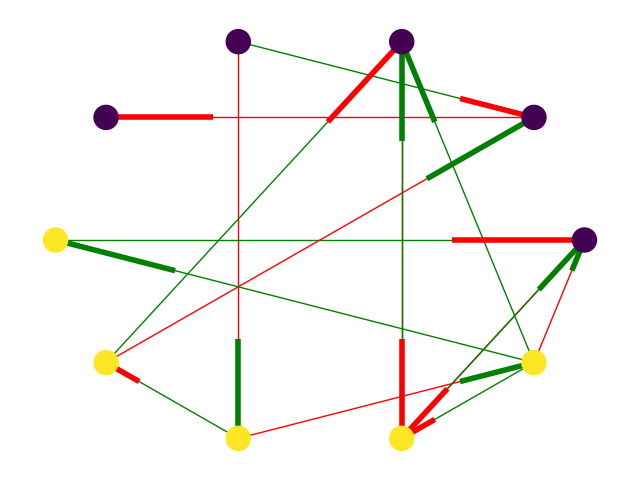
\includegraphics[width=\linewidth]{non-modular-example.png}
%		\caption{A non-modular example}
%	\end{subfigure}
%	\begin{subfigure}[b]{0.45\linewidth}
%		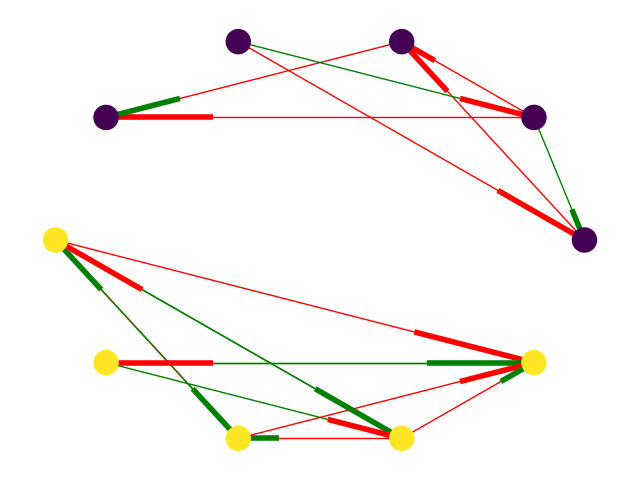
\includegraphics[width=\linewidth]{modular-example.png}
%		\caption{A modular example}
%	\end{subfigure}
%	\caption{Non-modular and modular networks}
%	\label{fig:network-example}
%\end{figure}
In the inception phase of this project, we utilized the Louvain heuristics to compute the partition of the network vertices in order to maximize the modularity of the given graph \cite{blondel2008fast}. We applied the tournament selection scheme with the tournament size being three and the elitism mechanism with ten elites in every generation. As a result of this setting, the partition of the gene regulatory networks by the Louvain heuristics demonstrated a very low modularity score. As Figure \ref{fig:early-modularity-not-work} indicates where the green line represents the generation to introduce specialization, by simulating the work in \cite{espinosa2010specialization}, we had expected there would be a spike after gene specialization on modularity. Nevertheless, we observed a modularity decrease as a result after gene specialization. 
\begin{figure}[h!]
	\centering
	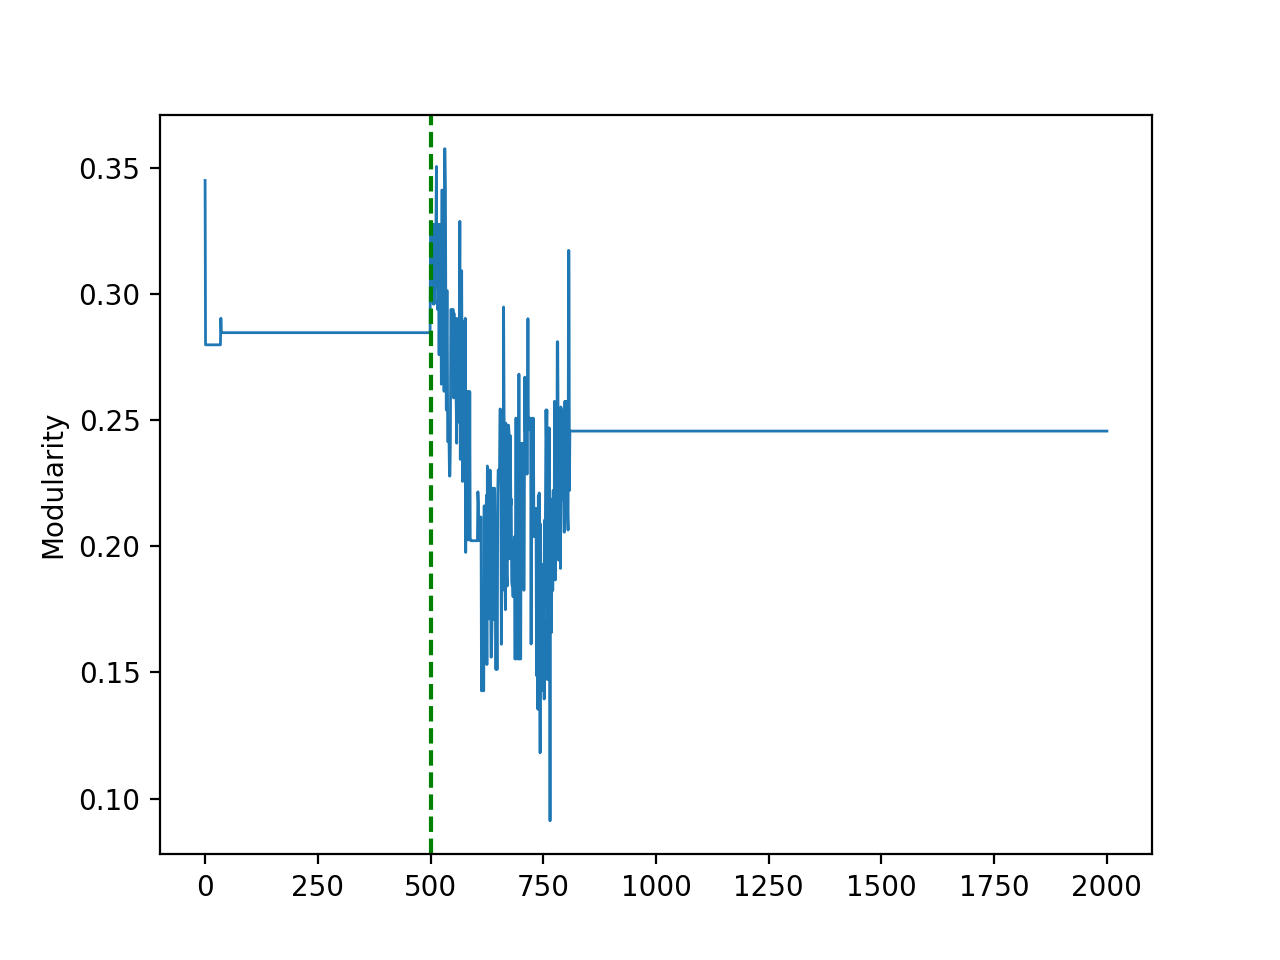
\includegraphics[width=\linewidth]{early-elitism-not-work.png}
	\caption{Modularity went worse after gene specialization}
	\label{fig:early-modularity-not-work}
\end{figure}
\begin{figure}[h!]
	\centering
	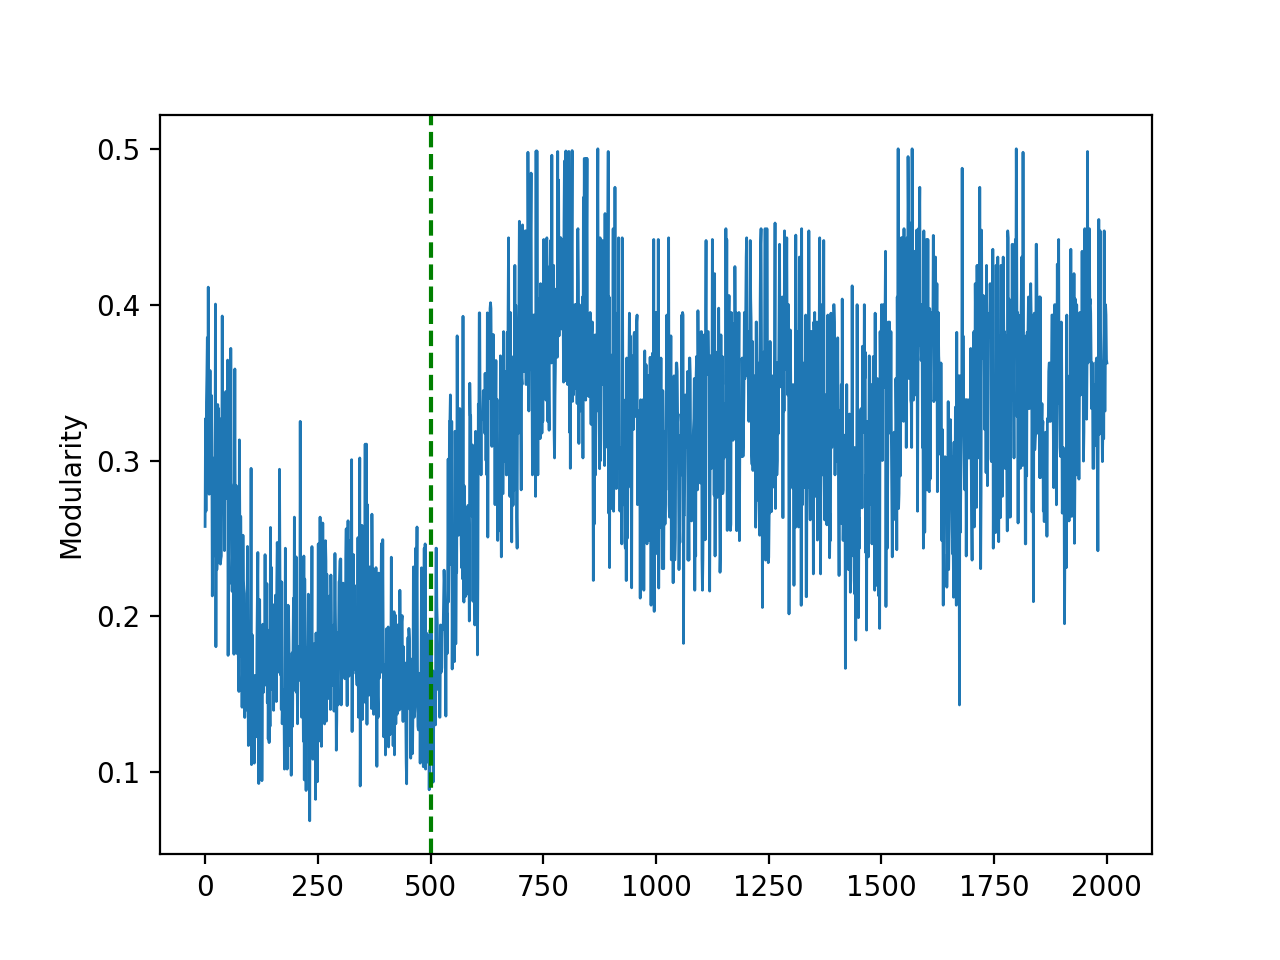
\includegraphics[width=\linewidth]{modularity-worked.png}
	\caption{Modularity emerged after gene specialization without elitism}
	\label{fig:modularity-worked-without-elitism}
\end{figure}
In order to understand this puzzling phenomenon, we removed the elitism mechanism and changed the tournament to proportional selection scheme. In consequence, we eliminated the deviant phenomenon as Figure \ref{fig:modularity-worked-without-elitism} indicates. Therefore, we hypothesized that the elitism mechanism or the tournament selection scheme hamper the evolutionary process on evolving out modular structures. 

